\section{球落下実験 実験結果}
\label{sec:expData}

本研究において,落下させる球の密度,擬塑性流体の質量濃度を変化させた.それぞれの質量濃度における,球の落下速度をFig.\ref{fig:0.05-0.2}-\ref{fig:1.5}に示す.横軸は経過時間[s],縦軸は落下速度[m/s]である.

\begin{figure}[h]
    \centering
    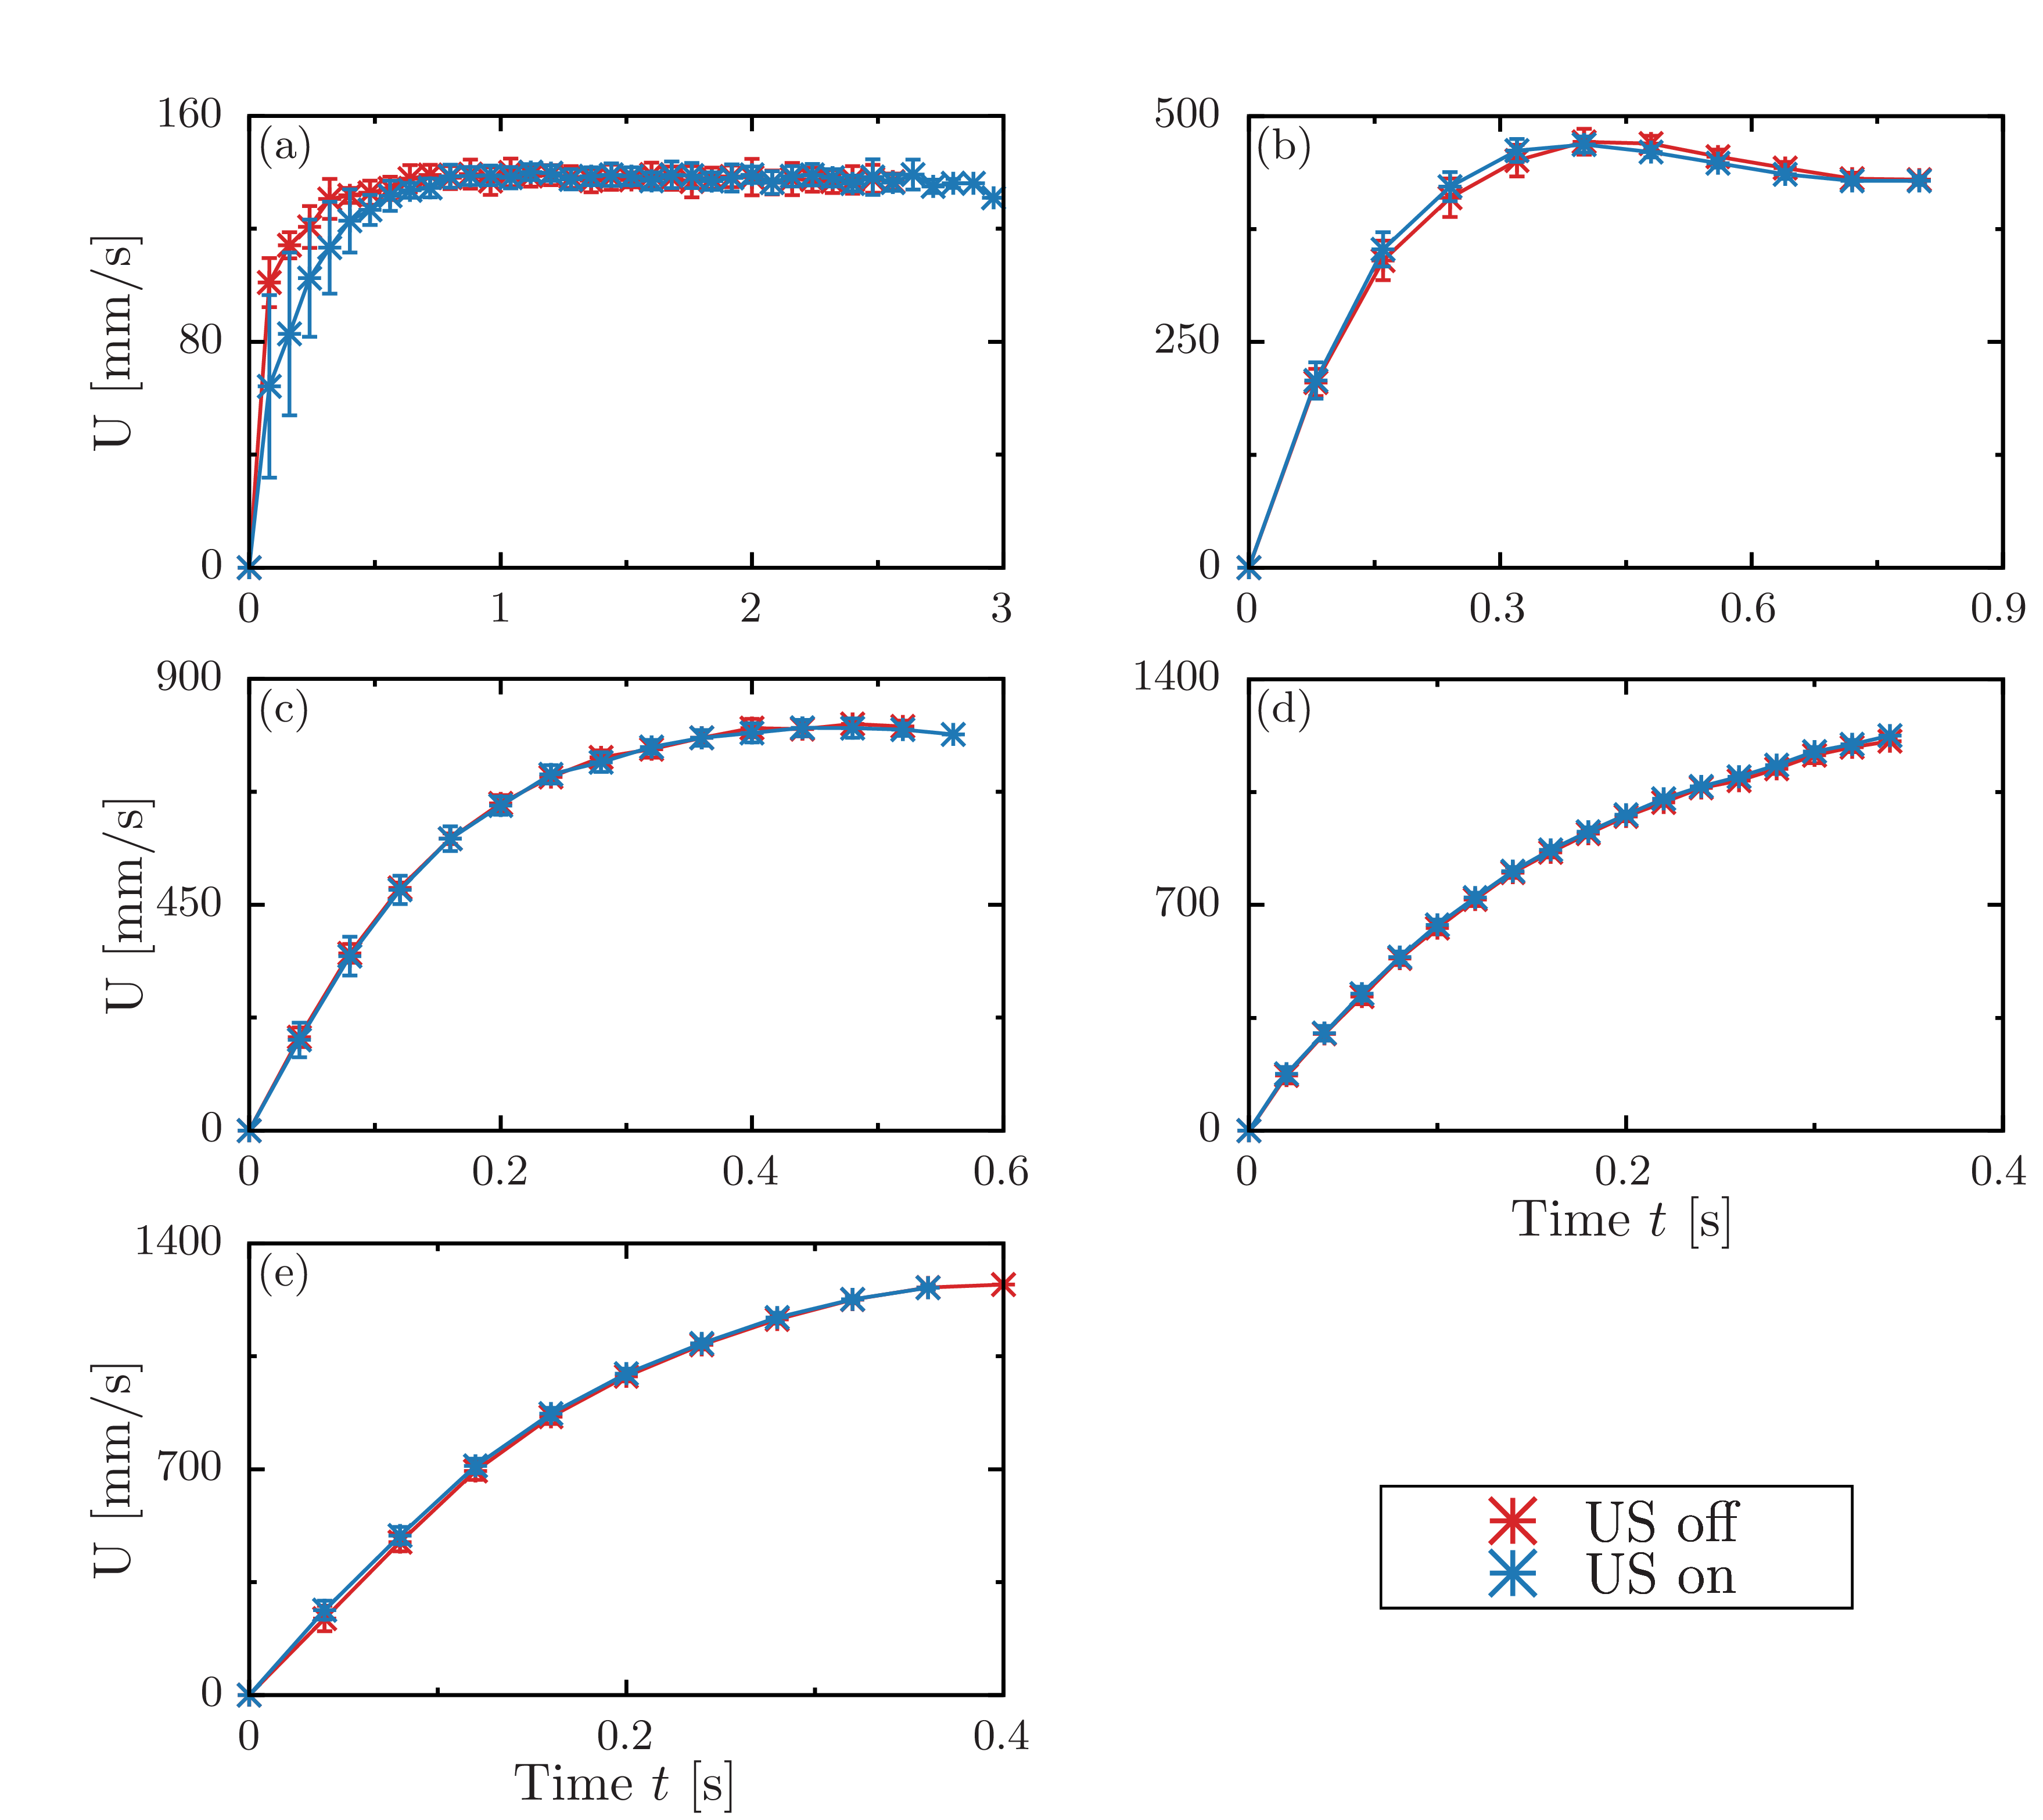
\includegraphics[width=15.0cm,clip]{5-Results/result_data/0.05-0.2.png}
    \caption{Velocity of a falling sphere made by (a)nylon in 0.05 wt.\% PAA solution, (b)aluminum, (c)alumina, (d)stainless,(e)brass in 0.2 wt.\% PAA solution.}
    \label{fig:0.05-0.2}
\end{figure}

\begin{figure}[h]
    \centering
    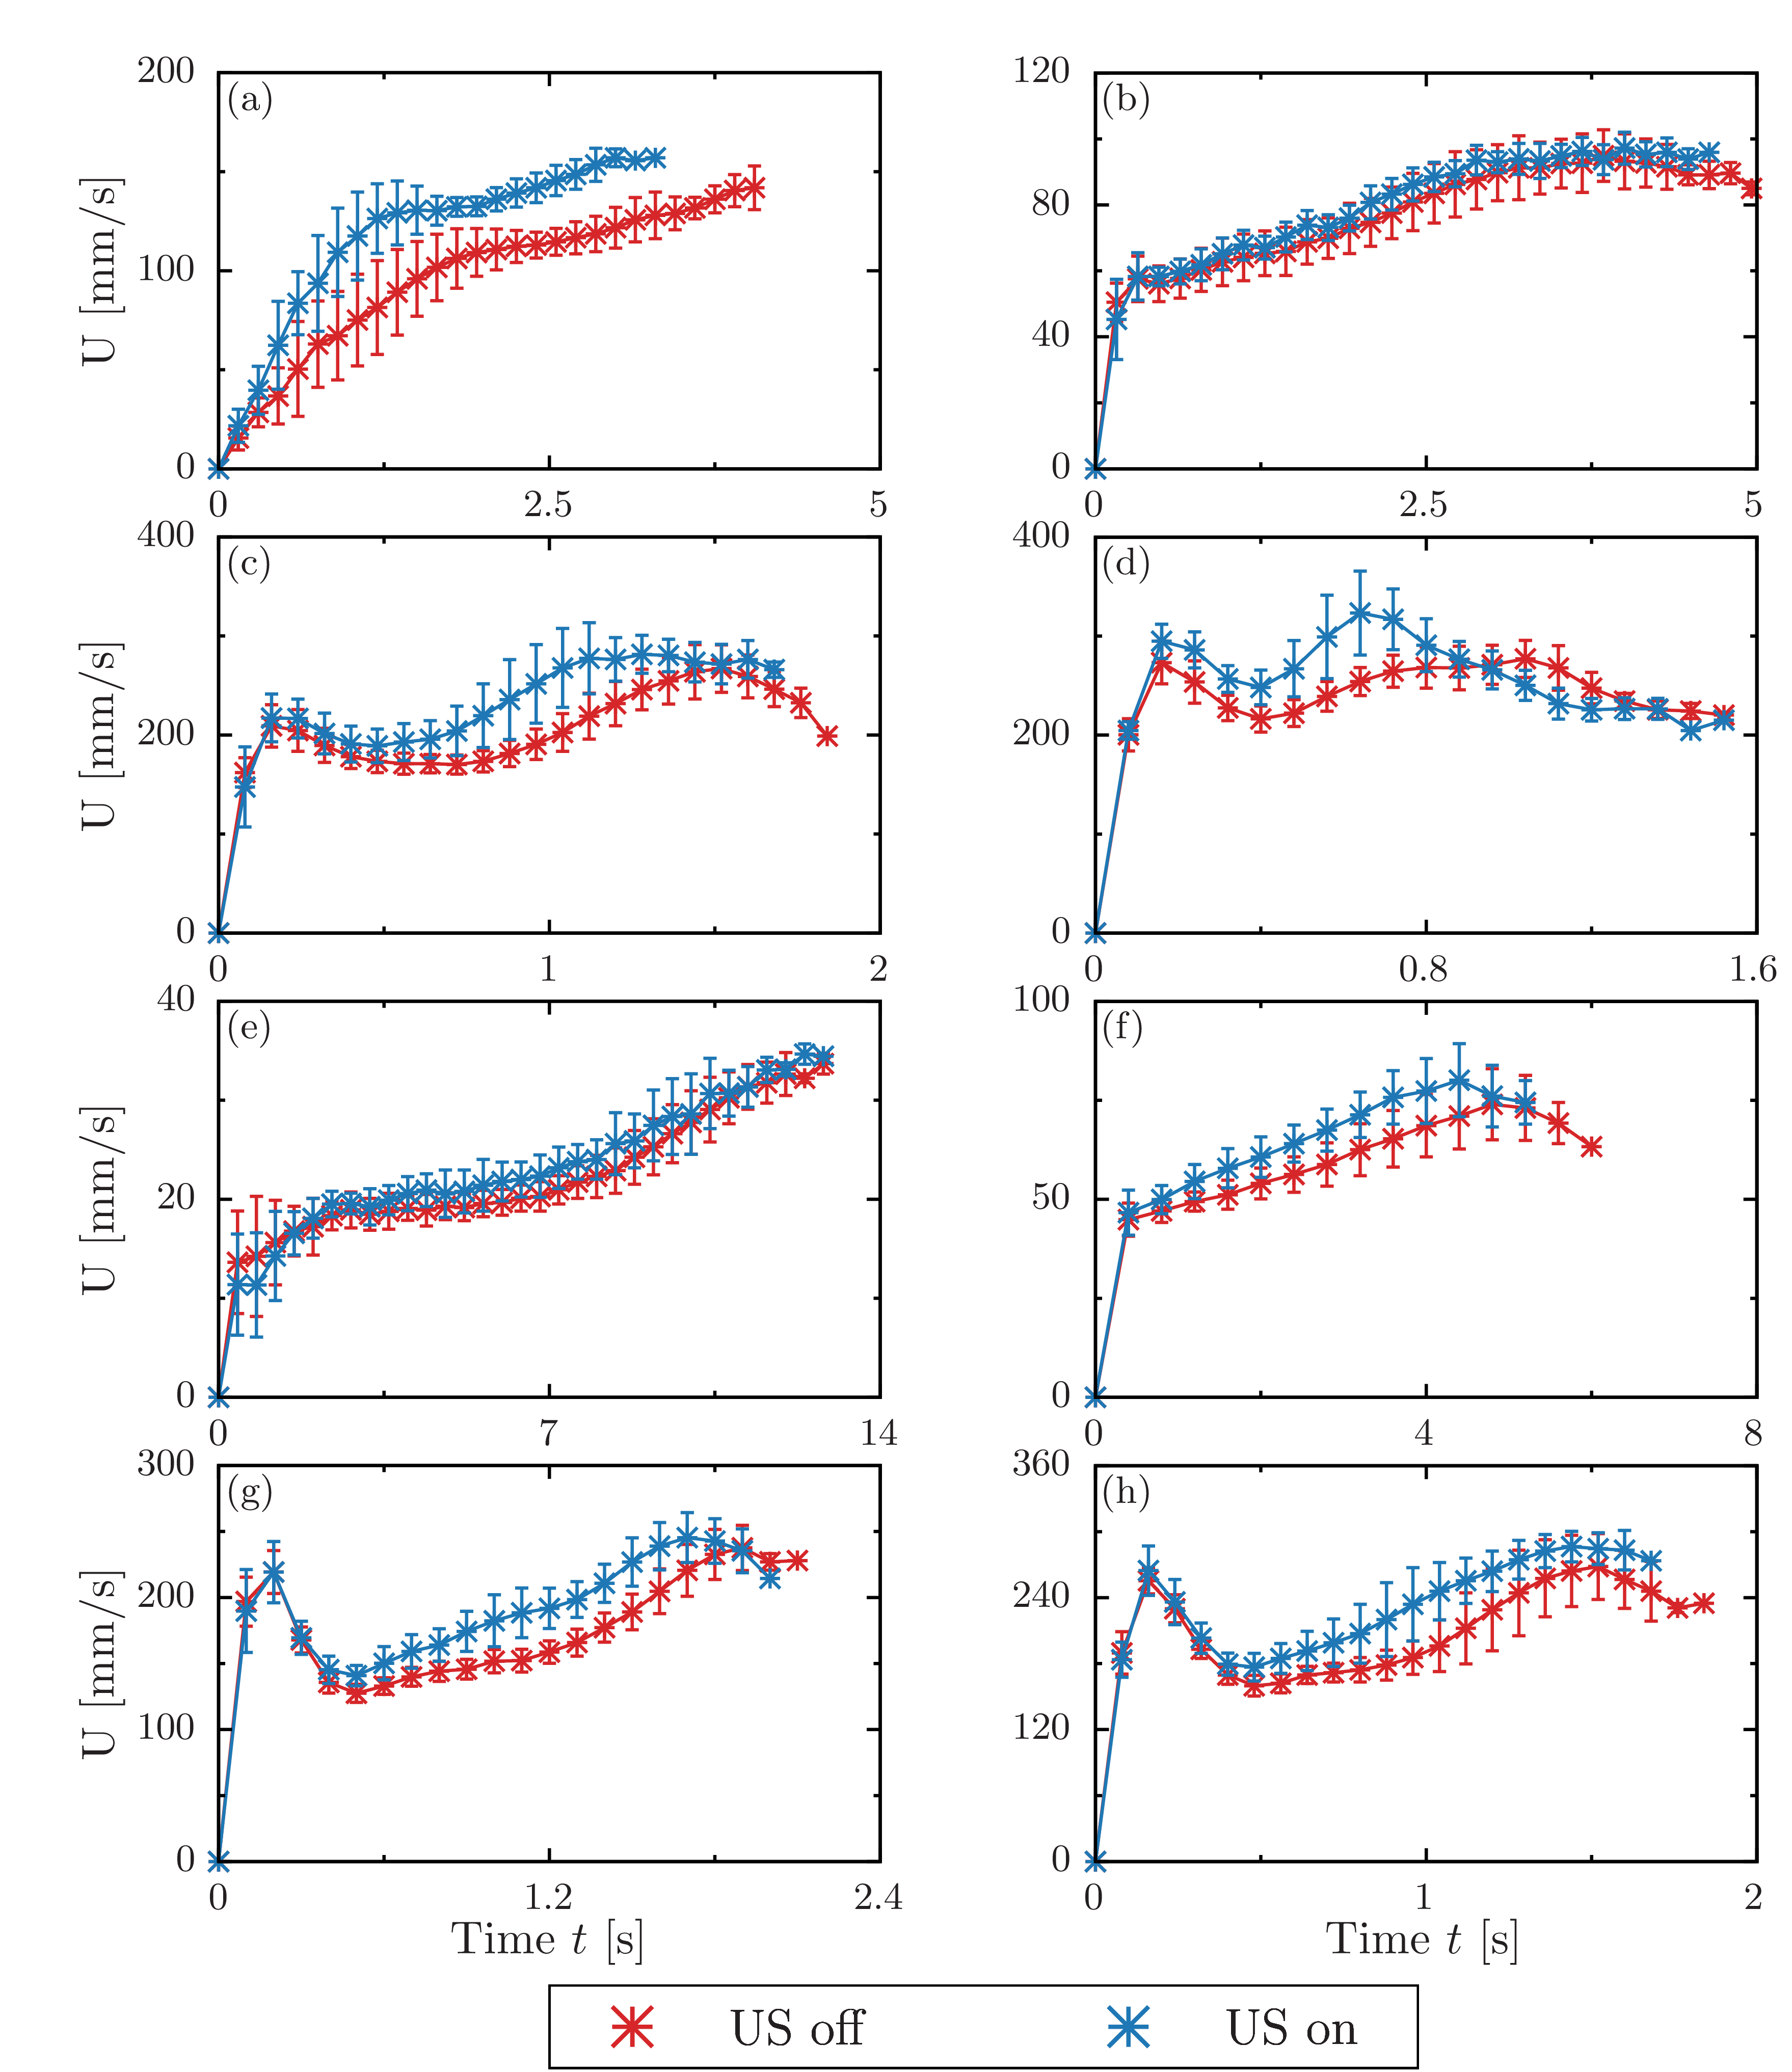
\includegraphics[width=15.0cm,clip]{5-Results/result_data/0.5-0.7.png}
    \caption{Velocity of a falling sphere made by (a)aluminum, (b)alumina, (c)stainless,(d)brass in 0.5 wt.\% PAA solution, (e)aluminum, (f)alumina, (g)stainless,(h)brass in 0.7 wt.\% PAA solution.}
    \label{fig:0.5-0.7}
\end{figure}

\begin{figure}[h]
    \centering
    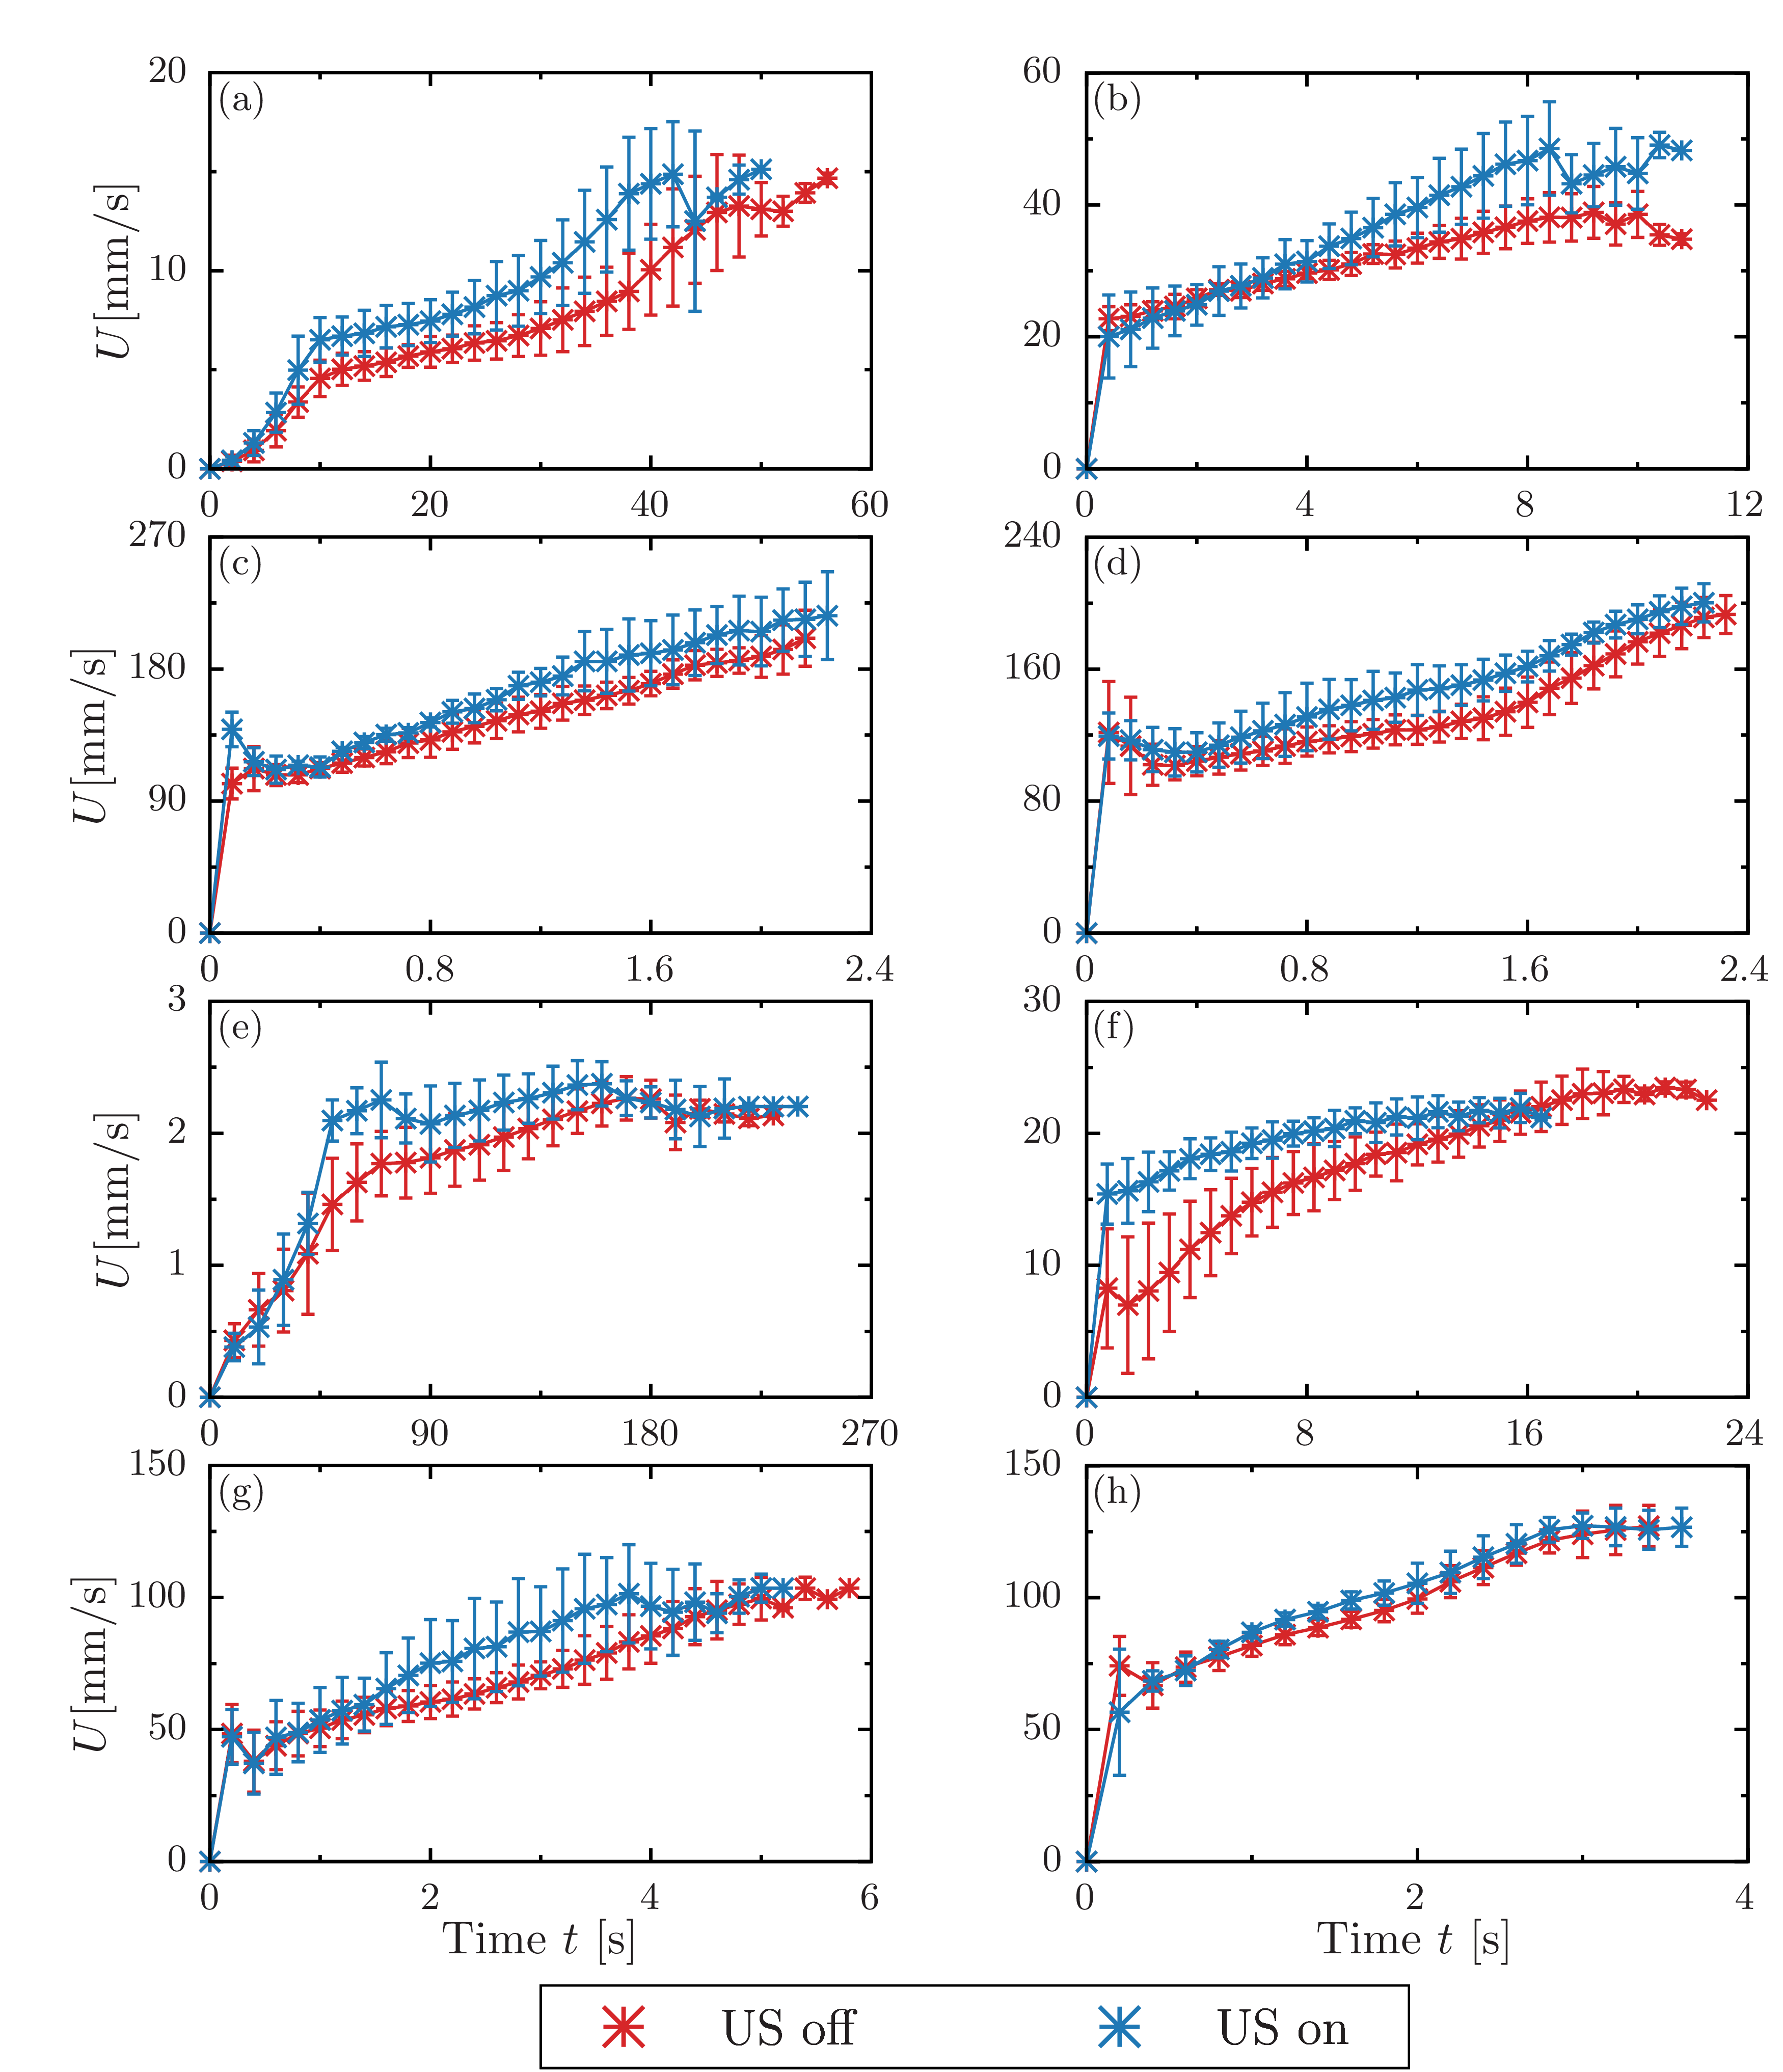
\includegraphics[width=15.0cm,clip]{5-Results/result_data/1.0-1.3.png}
    \caption{Velocity of a falling sphere made by (a)aluminum, (b)alumina, (c)stainless,(d)brass in 1.0 wt.\% PAA solution, (e)aluminum, (f)alumina, (g)stainless,(h)brass in 1.3 wt.\% PAA solution.}
    \label{fig:1.0-1.3}
\end{figure}

\begin{figure}[h]
    \centering
    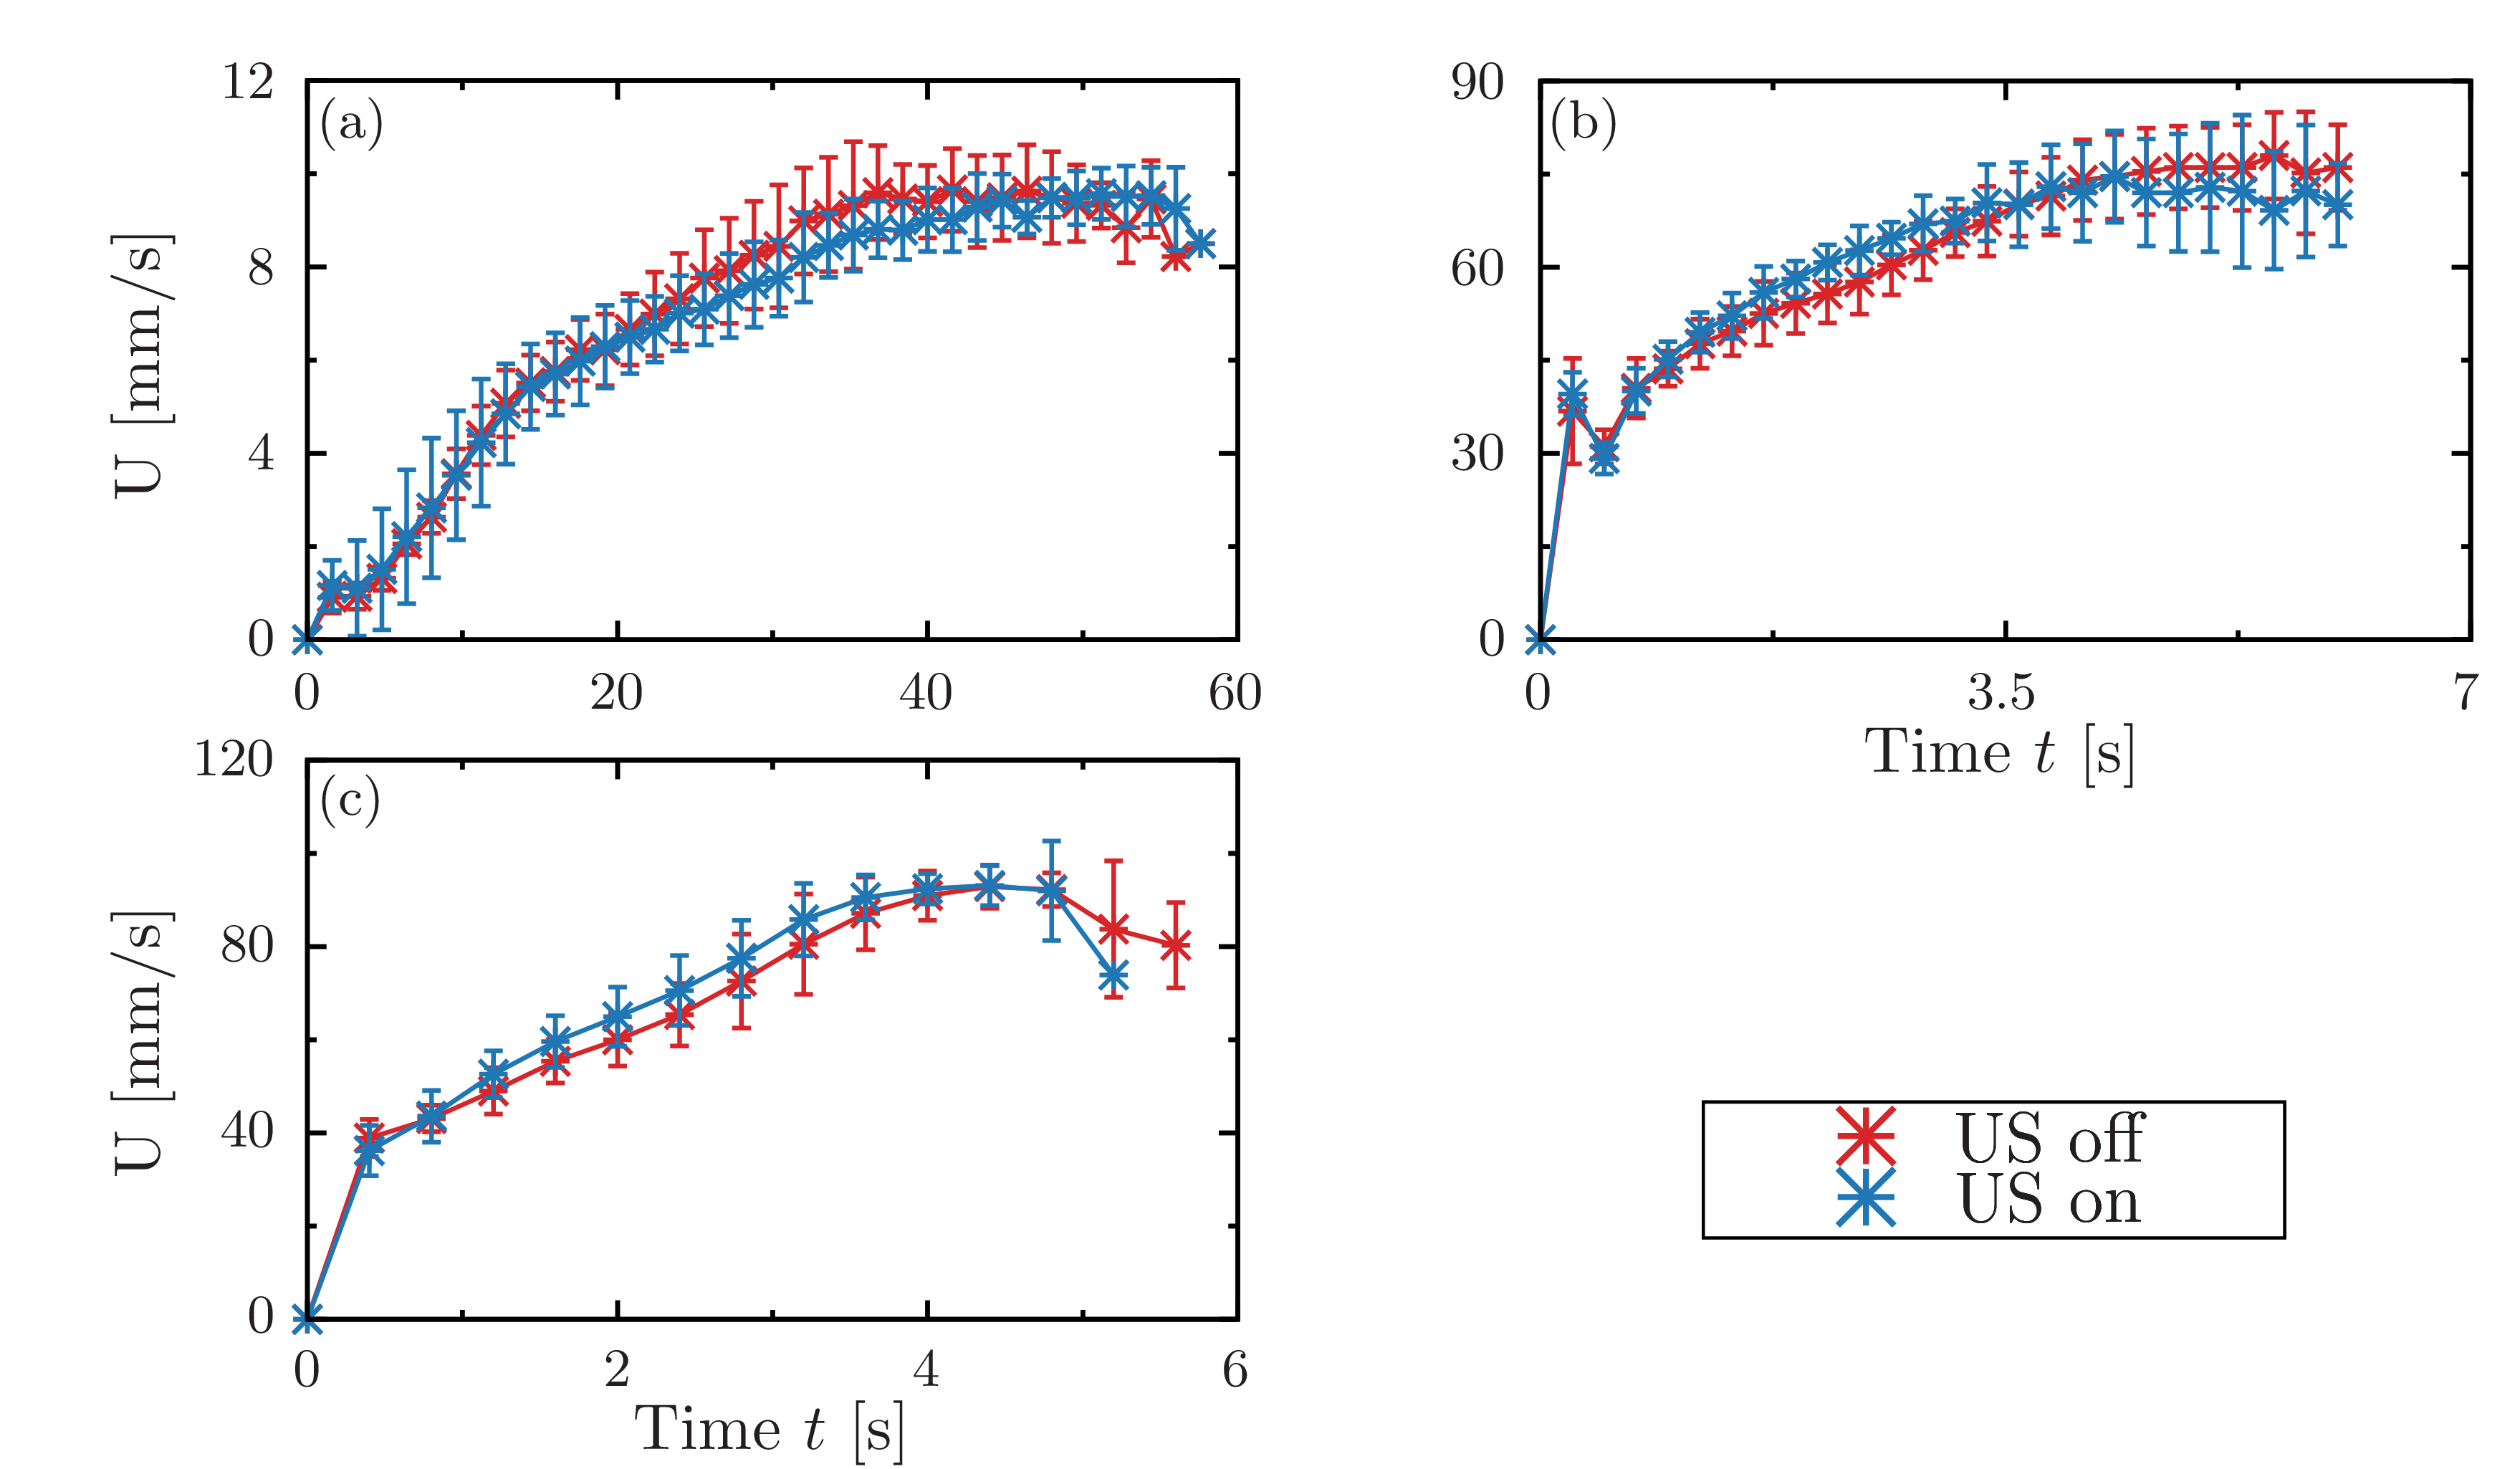
\includegraphics[width=15.0cm,clip]{5-Results/result_data/1.5.png}
    \caption{Velocity of a falling sphere made by (a)alumina, (b)stainless,(c)brass in 1.5 wt.\% PAA solution.}
    \label{fig:1.5}
\end{figure}